\begin{CJK}{Bg5}{bsmi}

%---------------------------------------------
%	Chapter System Architecture
%---------------------------------------------

\chapter{System Architecture}

In this chapter, I am going to explain my design more detailed. My scheme is based on DSA to provide the security and I'll explain it in the first section. The second section exhibits the user flow in three phases: \emph{register}, \emph{login} and \emph{verification}.

\section{System Overview}

Let us recall the authentication process about the password-based scheme. As the fig~\ref{fig:password-based-flow} shows, the client give his username and password to server, note that the password must to be encrypted because of the security issue. Then the verification server checks whether it is valid according to its database and return the result to user. Figure~\ref{fig:my-scheme-flow} is the authentication process of my scheme. Client should send a login request first, because the verification server is a passive element. After receive a login request, the server will send a nonce, which is composed by the server information and some random bits, back to the client. The client generates a signature for this nonce and return to server. The server uses the public key to check whether the client is valid or not.

In comparison to the password-based scheme, my scheme needs two extra steps. But it is not an big issue due to the high data transfer speed of NFC technique. According to this concept, the advantage is that the data communicated between the client and the server doesn't need to be encrypted. The only \emph{secret} is private key, which is stored in client's storage. The disadvantage of my scheme is that users will need to hold a device for creating signature and help them managing their public keys. The next section will offer introduction for each components.
\begin{figure}
\centering
\subfigure[password-based scheme]{
\label{fig:password-based-flow}
\includegraphics[scale=0.6]{picture/password-based-flow.png}
}
\subfigure[my scheme]{
\label{fig:my-scheme-flow}
\includegraphics[scale=0.6]{picture/basic-idea-flow.png}
}
\caption{Authentication flow}
\end{figure}

\begin{figure}
\centering
\includegraphics[scale=0.65]{picture/final-flow.png}
\caption{Authentication flow with mobile device}
\label{fig:final-flow}
\end{figure}

\section{Components and Data flow}

There are 5 parts of my scheme: \emph{Mobile device}, \emph{NFC reader application}, \emph{browser}, \emph{srever} and \emph{its database}, as the figure shows. In this section, I'll introduce the envienment I setup for this system.

\subsubsection{Mobile Device and NFC Channel}

For the mobile device, I use Nesus7 with Android OS (version = 4.4) in my experiments. Android OS provide a HostApduService for developers to manage the NFC communication. Specifically, Android 4.4 supports emulating cards that are based on the NFC-Forum ISO-DEP specification (based on ISO/IEC 14443-4) and process Application Protocol Data Units (APDUs) as defined in the ISO/IEC 7816-4 specification. The protocol stack shows as fig~\ref{fig:protocol-stack}. When the user taps a device to an NFC reader, the Android system needs to know which HCE service the NFC reader actually wants to talk to. This is where the ISO/IEC 7816-4 specification comes in: it defines a way to select applications, centered around a 16-bytes Application ID (AID).

\begin{figure}
\centering
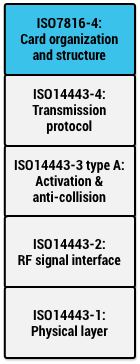
\includegraphics[scale=0.7]{picture/protocol-stack.png}
\caption{Android's HCE protocol stack\cite{nfc-hce-stack}}
\label{fig:protocol-stack}
\end{figure}

\subsubsection{Browser and NFC Reader}
In my setup, it doesn't need a specify browser. Some common browser such as Google Chrome, FireFox or even IE can support this scheme. The NFC reader I used is ACR122U. The browser connect to NFC reader through Libnfc\cite{libnfc}, a open-source project about developing NFC-related application.

\subsubsection{Server and its Database}

I use flask, a python framework for web application, for building an verification server in order to proof my concept. I choose to use SQL database, which means my scheme are compatible to password-based scheme. I use HTTP as the transmission protocol. The reason why I don't use HTTP is because of my threat model assumption. I assume that the client side (browser and NFC reader) is unsecure, so even though I adopt HTTPS, the certificate is still untrusted. Thus, I select an unsecure transmission protocol to emphasize that the client-side is untrusted.

\section{User Flow}

In this section, I'll separate the authentication process into three stages: \emph{register phase}, \emph{login phase} and \emph{verification phase}.

\subsubsection{Register Phase}

\begin{enumerate}
\item Start the initialization process on his mobile device, that is, set PIN code and generate key pair.
\item User send a registration request to the verification server.
\item Server return the server information to user and pass it to mobile device via reader application.
\item Mobile device saved the server information and the private key together, and return the device UUID and corresponding public key back to user.
\item User send the id and public key (and other required credentials required by server) to server.
\item Server saved UUID and public key into its database.
\end{enumerate}

In step one, users need to set a PIN code in order to resist to theft. The key pair is generated by RSA in my implementation, but it can be replaced with any other asymmetric key encryption algorithm. In step three, the reason why the server has to add server info into the nonce is to resist to the Man-In-The-Middle attack. In step four, I take the device UUID as the identifier instead of the public key is because there are various kinds of DSA, I have to unite the ID format for all the users and all the devices.

\subsubsection{Login Phase}

\begin{enumerate}
\item User send a login request to server.
\item Server return a nonce ([server info || random bits]) back to client.
\item The NFC reader start to scan cards as soon as it receive the nonce.
\item User execute the card emulation application on mobile device and enter the PIN code. If the PIN code correct, mobile device enable the HCE mode.
\item Reader application send nonce to mobile device.
\item Mobile device retrieve the server info from nonce, show it on the screen and ask for user's confirmation.
\item Mobile device signed the nonce with corresponding private key.
\item Mobile device pass its UUID and signed-nonce to reader.
\item Client pass these parameters to server.
\end{enumerate}

Note that users have to swipe their device to the NFC reader in 30 seconds right after the reader start scanning. Otherwise, it will send a timeout message to browser. In step nine, verification server is able to ask user to provide some other credentials, but we will not discuss about that because it is not defined in my scheme.

\subsubsection{Verification Phase}

\begin{enumerate}
\item Server retrieve the corresponding public key according to the UUID.
\item Verify the signature with the public key.
\item Return the verification result back to client.
\end{enumerate}

\begin{comment}
\section{Scenario}

\subsection{Future Website}
\label{sec:future-website}

\subsection{Existing Website}

For existing website, it is difficult for them to integrate this scheme with their origin users. Therefore, they can adopt the OpenID protocol to help. Build a verification server with this new scheme and use it to be the \emph{Relying Party} in OpenID protocol.

Take Bitcucket.org as an example, I modified the verification server in section~\ref{sec:future-website} to be an \emph{openid-provider}, that is, to support OpenID feature. When a user need to login to Bitbucket, he have to switch to openid-login mode, enter the server url. Then the authentication process is as same as I described above. 
\end{comment}

\end{CJK}